%%%% fatec-article.tex, 2024/03/10

%% Classe de documento
\documentclass[
  a4paper,%% Tamanho de papel: a4paper, letterpaper (^), etc.
  12pt,%% Tamanho de fonte: 10pt (^), 11pt, 12pt, etc.
  english,%% Idioma secundário (penúltimo) (>)
  brazilian,%% Idioma primário (último) (>)
]{article}

%% Pacotes utilizados
\usepackage[]{fatec-article}
\usepackage{float}
\usepackage{amsmath} 
\Author{1}{Name={Amanda de Oliveira Costa\\ Arthur Ribeiro Dias Fudali \\ Giovana da Silva Albanês Santos }}

\Author{2}{Name={\{ amanda.costa47@fatec.sp.gov.br \}\\ \{ arthur.fudali@fatec.sp.gov.br \} \\ \{ giovana.santos30@fatec.sp.gov.br\}}}

%% Definição das palavras-chaves/keywords
\Keyword{1}{UI/UX}{UI/UX}
\Keyword{2}{Validação de Design}{Design Validation}
\Keyword{3}{Rastreamento Ocular}{Eye Tracking}
\Keyword{4}{Inteligência Artificial}{Artificial Intelligence}
\Keyword{5}{Heatmap}{Heatmap}
\Keyword{6}{Feedback Visual}{Visual Feedback}
\Keyword{7}{Análise Comportamental}{Behavioral Analysis}
\Keyword{8}{Experiência do Usuário}{User Experience}
\Keyword{9}{Predição de Heatmap}{Heatmap Prediction}
\Keyword{10}{Otimização Contínua}{Continuous Optimization}

%%%% Resumo no idioma primário (brazilian)
\begin{Abstract}[brazilian]%% Idioma (brazilian ou english)
  A criação de interfaces UI/UX eficazes depende de uma validação cuidadosa que assegure o alinhamento com as expectativas e necessidades dos usuários. Contudo, muitos designers enfrentam desafios em obter feedback visual preciso e em tempo real, essencial para aprimorar a experiência do usuário. O Ueye busca solucionar esse problema ao combinar rastreamento ocular (Eye Tracking) e inteligência artificial (IA), facilitando a análise visual de interfaces e auxiliando designers a identificar áreas de atenção e desinteresse com maior precisão. Através do sistema de Eye Tracking, os usuários podem interagir com o design enquanto o ponto de foco visual é registrado em uma matriz de atenção, que agrega valores em cada área onde o olhar se fixa. Esse processo gera heatmaps que indicam as regiões de maior e menor interesse visual, fornecendo aos designers uma base sólida para otimizar a disposição dos elementos visuais. Os heatmaps gerados não apenas orientam ajustes de design, mas também alimentam a IA do Ueye, que aprende padrões de comportamento visual a partir de múltiplas interações. Isso permite que a IA faça previsões automáticas de heatmap para novos designs, antecipando os pontos de interesse visual sem a necessidade de testes adicionais.  Esse sistema representa um avanço significativo para o design de interfaces, fornecendo uma ferramenta poderosa que integra feedback em tempo real e predições automáticas, permitindo que designers façam melhorias contínuas com base em dados confiáveis. Ao unir Eye Tracking e inteligência artificial, o Ueye proporciona uma análise detalhada do comportamento do usuário, garantindo que as interfaces sejam não apenas visualmente atraentes, mas também altamente funcionais. 
\end{Abstract}

%%%% Resumo no idioma secundário (engl  ish)
\begin{Abstract}[english]%% Idioma (brazilian ou english)
  Creating effective UI/UX interfaces relies on careful validation to ensure alignment with user expectations and needs. However, many designers face challenges in obtaining accurate, real-time visual feedback, which is essential to improving the user experience. Ueye aims to solve this problem by combining eye tracking and artificial intelligence (AI), facilitating visual analysis of interfaces and helping designers identify areas of attention and disinterest with greater precision. Through the Eye Tracking system, users can interact with the design while the visual focus point is recorded in an attention matrix, which aggregates values in each area where the gaze is fixed. This process generates heatmaps that indicate the regions of greatest and least visual interest, providing designers with a solid basis for optimizing the placement of visual elements. The generated heatmaps not only guide design adjustments, but also feed Ueye's AI, which learns patterns of visual behavior from multiple interactions. This enables AI to automatically make heatmap predictions for new designs, anticipating visual interest points without the need for additional testing. This system represents a significant advancement for interface design, providing a powerful tool that integrates real-time feedback and automatic predictions, allowing designers to make continuous improvements based on reliable data. By combining Eye Tracking and AI, Ueye provides detailed analysis of user behavior, ensuring that interfaces are not only visually appealing, but also highly functional.
\end{Abstract}

%% Processamento de entradas (itens) do índice remissivo (makeindex)
\makeindex%

%% Arquivo(s) de referências
\addbibresource{fatec-article.bib}

%% Início do documento
\begin{document}

% Seções e subseções
%\section{Título de Seção Primária}%

%\subsection{Título de Seção Secundária}%

%\subsubsection{Título de Seção Terciária}%

%\paragraph{Título de seção quaternária}%

%\subparagraph{Título de seção quinária}%

\section*{Introdução}%
\label{sect:intro}
A Organização das Nações Unidas (ONU) é uma instituição que visa estabelecer a paz, segurança e desenvolvimento global. A ONU conta com 193 países-membros que formam a Assembleia Geral, responsável por desenvolver as políticas da organização. Em 2015, como parte da Agenda 2030 para o Desenvolvimento Sustentável, foram criados 17 objetivos que abrangem desde a melhoria da indústria até o aprimoramento da saúde da população. Esse conjunto de metas constitui um plano de ação ambicioso para as pessoas, o planeta e a prosperidade. Este trabalho visa contribuir para o nono objetivo, que promove Inovação e Infraestrutura, ao desenvolver uma nova abordagem para analisar o design de interfaces de usuário.
\textcite{ODS2024}

As Interfaces de Usuário (UI) e a Experiência de Usuário (UX) são elementos fundamentais na interação entre um cliente e um produto digital. Essas duas áreas do design, quando combinadas, desempenham um papel crucial na satisfação do usuário com um sistema. A UI tem como foco a criação e melhoria dos aspectos visuais e interativos do produto. Seu objetivo é tornar a interface esteticamente agradável e funcional, facilitando uma interação mais eficiente e intuitiva entre o usuário e o produto.

Por outro lado, a UX abrange uma área maior dentro do Design, considerando todos os aspectos da interação do usuário com o produto, como a intuitividade do sistema e as emoções sentidas durante a utilização. Juntas, UI e UX trabalham em sinergia para criar uma experiência de uso satisfatória que atenda aos requisitos funcionais do usuário de forma simples e eficaz. 
\textcite{EBAC}

A experiência proporcionada pela UI é de extrema importância para o sucesso de um produto digital no mercado atual, altamente competitivo e centrado no usuário. Uma interface que seja simultaneamente funcional, esteticamente atraente e intuitiva de usar torna-se um fator decisivo na adoção inicial e na fidelização a longo prazo do usuário ao produto. Além disso, uma UI bem projetada pode significativamente reduzir a curva de aprendizado, minimizar erros do usuário, aumentar a eficiência nas tarefas e, consequentemente, elevar os níveis de satisfação e produtividade do usuário. Portanto, investir no desenvolvimento de uma UI de alta qualidade não é apenas uma questão de estética, mas uma estratégia fundamental para o sucesso e a sustentabilidade de qualquer produto digital no cenário tecnológico contemporâneo.

O teste da interface de usuário é frequentemente conduzido através de um procedimento conhecido como Teste de Usabilidade. Este método de avaliação consiste em uma entrevista estruturada, realizada em um ambiente controlado, onde há uma interação direta entre o pesquisador e o usuário de teste. Durante essa sessão, a atenção é dedicada principalmente às características específicas de uso e às funcionalidades específicas da interface em questão.

O objetivo deste tipo de teste é realizar uma análise do comportamento do usuário enquanto ele interage com o produto digital. Isso inclui observar como o usuário navega pela interface, quais elementos chamam sua atenção, onde encontra dificuldades e como resolve problemas. Além disso, o teste busca coletar informações sobre a eficiência com que o usuário realiza tarefas específicas, o tempo necessário para completá-las e o nível de satisfação geral com a experiência de uso.

Através deste processo, os pesquisadores podem identificar pontos fortes e fracos na interface, detectar possíveis obstáculos na experiência do usuário e coletar informações valiosas para futuras melhorias. Esta abordagem permite que as equipes de design e desenvolvimento refinem continuamente a interface, garantindo que ela atenda às necessidades do usuário e as expectativas relacionadas a qualidade de uso do sistema.

Essa análise é realizada considerando fatores como: o tempo que o usuário permanece em cada tela, o número de etapas necessárias para realizar uma tarefa, a quantidade de erros cometidos durante o processo e as sensações experimentadas ao usar o sistema. Tal avaliação detalhada só é possível quando um pesquisador observa atentamente cada passo do usuário. Por outro lado, numa análise não moderada — isto é, sem supervisão direta — o resultado pode ser comprometido, pois depende exclusivamente do feedback fornecido pelo usuário, e não de métricas objetivamente coletadas. Essa limitação afeta tanto a profundidade da análise quanto a credibilidade do teste.

\textcite{BELISIARIO2023, VIEIRA2019}


O eye tracking é uma técnica que consiste em usar o posicionamento dos olhos de uma pessoa para obter informações sobre onde ela está olhando. Isso pode ser feito usando luzes infravermelhas, que calculam exatamente onde a pessoa está olhando com base nas reflexões da luz na retina, ou por meio de câmeras que monitoram visualmente a posição dos olhos e identificam sua direção.

Quando aplicada a um teste de usabilidade, essa tecnologia pode fornecer insights valiosos ao pesquisador. Ela permite saber com precisão onde o usuário está olhando, o que ele procura e por quanto tempo olhou para cada elemento. Isso possibilita identificar problemas como textos confusos ou mal formatados, ou até mesmo elementos visuais que chamam atenção indevidamente e diferem da identidade visual do sistema, prejudicando sua usabilidade.

Assim, propomos por meio deste estudo a criação de um software (uEye) que usa as informações obtidas pelo rastreamento ocular de usuários durante o uso de telas de um sistema. Essas informações serão usadas para treinar uma inteligência artificial capaz de identificar, de forma rápida e precisa, possíveis divergências na Interface de Usuário de um sistema que poderiam prejudicar a Experiência do Usuário durante o uso.




\section*{OBJETIVO} \label{sect:obj}

\subsection*{1. OBJETIVO GERAL}
Desenvolver um sistema inteligente de eye tracking que auxilie designers de experiência do usuário (UX) na otimização de interfaces gráficas. O sistema utilizará técnicas de visão computacional para capturar o comportamento visual dos usuários, gravando onde eles olham para formar mapas de calor que evidenciam as áreas de maior atenção e interação. O objetivo é antecipar ajustes necessários e aprimorar o processo de design, oferecendo dados precisos sobre a interação do usuário com a interface.

\subsection*{2. OBJETIVOS ESPECIFICOS}
\begin{enumerate}
    \item Aplicar técnicas de visão computacional para capturar e analisar o comportamento visual dos usuários durante a interação com a interface.
    \item Criar um módulo que permita a realização de testes com usuários reais, incluindo a captura do comportamento visual por meio de visão computacional durante o uso da interface.
    \item Criar algoritmos que transformem os dados de eye tracking em heatmaps, visualizando as áreas de maior atenção e interação dos usuários nos designs analisados.
    \item Realizar análises estatísticas e qualitativas dos dados coletados para entender como os usuários interagem com os elementos da interface, identificando padrões de comportamento.
    \item Implementar uma funcionalidade que permita o upload de designs, possibilitando que a inteligência artificial analise os dados.
    \item Desenvolver um modelo de inteligência artificial em Python, capaz de gerar avaliações sobre o design com base nas interações visuais dos usuários e aprendizado prévio.
    \item Otimizar o trabalho do UX designer, desenvolvendo um modelo de inteligência artificial capaz de gerar heatmaps nas telas enviadas.
    \item Implementar um módulo para visualizar as avaliações e heatmaps dos designs enviados para a inteligência artificial.
    \item Implementar um módulo que permita visualizar as avaliações e heatmaps dos designs analisados através de eye tracking.
    \item Criar gráficos que compilem e apresentem a distribuição das notas baixas atribuídas pela inteligência artificial em diferentes quesitos, oferecendo insights sobre áreas a serem melhoradas.
    \item Produzir gráficos que ilustrem a taxa de satisfação que a IA supõe que os clientes teriam em resposta a melhorias no design, variando de insatisfeito a satisfeito.
    \item Conduzir testes de usabilidade para validar a eficácia do sistema de eye tracking e avaliações por inteligência artificial, coletando feedback dos usuários para ajustes e melhorias.
    \item Documentar os resultados obtidos durante a pesquisa, incluindo o impacto da análise dos heatmaps e avaliações preditivas na experiência do usuário.
\end{enumerate}








\section*{ESTADO DA ARTE} \label{sect:estadoarte}

Nesta seção, você deverá realizar um mapeamento de toda a produção acadêmica sobre o tema do seu projeto. É um processo bastante importante porque reúnem todas as pesquisas e descrevem as conclusões das pesquisas sobre o tema \cite{smith:99}. Para escrever um bom estado da arte, você poderá utilizar algumas perguntas norteadoras, tais como:

\begin{enumerate}
    \item O que as atuais pesquisas científicas concluíram sobre o tema?
    \item Quais as divergências dos pesquisadores sobre o assunto?
    \item Quem está pesquisando sobre esse tema?
    \item Onde estão fazendo essas pesquisas?
\end{enumerate}

Em outras palavras, o estado da arte destaca os aspectos de outras pesquisas, mas também identifica as lacunas que existem nessas pesquisas. Ou seja: analisa o que as pesquisas falaram e o que não falaram sobre o tema \cite{Alencar2007,Beltrano2021,Fulano2021}.

Segundo \textcite{Ramos2003,Carvalho2004}, para que você possa descrever as pesquisas/trabalhos que estão relacionados ao seu, não esqueça de citá-los ao decorrer do texto. Para isso, você poderá utilizar o comando $\backslash$cite para citação implícita ou o comando $\backslash$textcite para citações explícitas.

As citações diretas curtas (de até três linhas) acompanham o corpo do texto e se destacam com aspas duplas. Caso o texto original já contenha aspas, estas devem ser substituídas por aspas simples. Enquanto que, para representar as citações diretas longas (com mais de três linhas), estas devem ser transcritas em parágrafo distinto, da seguinte forma:

\begin{displayquote}
   Toda citação direta com mais de três linhas é considerada uma citação direta longa.
Este tipo de citação deve ser escrita sem aspas, em parágrafo distinto, com fonte de tamanho 10, espaçamento simples e com recuo de 4cm da margem esquerda, terminando na margem direita, conforme ilustrado neste exemplo \cite{Andujar2006}.
\end{displayquote}

Vale ressaltar que a utilização de citações diretas longas deve ser evitada durante a escrita de artigos científicos. Conforme visto em \textcite{Kalakota2002,Purcidonio2008}, os dados de cada referência podem ser obtidos de um arquivo com a extensão bib, geralmente na própria página de \textit{download} da referência (artigos, livros, etc.) ou, ainda, a partir do Google Acadêmico, etc.



\section*{METODOLOGIA} \label{sect:metodologia}

O projeto visa desenvolver uma ferramenta web de apoio aos designers de UX, que integra Eye Tracking, HeatMaps e Inteligência Artificial para auxiliar na validação de interfaces. O foco principal do sistema é o designer, permitindo ao cliente participar apenas da fase de rastreamento ocular, quando necessário.

O método proposto baseia-se na construção de um sistema web destinado aos designers de UX, oferecendo a possibilidade de consulta à IA para análise preditiva. Neste processo, o designer pode enviar uma tela para a IA, que retorna um heatmap e uma escala de satisfação de 1 a 5, considerando quatro critérios principais: usabilidade, atratividade visual, clareza das informações e fluxo da navegação.

Para que a IA possa oferecer essas análises, é necessário alimentá-la com dados derivados de uma matriz de rastreamento ocular, que armazena a frequência e a intensidade do foco visual durante os testes. A coleta desses dados ocorre quando o cliente interage com a interface sendo testada, enquanto o sistema de Eye Tracking executa em segundo plano. A matriz registra a intensidade do olhar em diferentes áreas da tela, indicando as regiões de maior e menor interesse.

Ao final do teste, esses valores são processados para gerar o heatmap da tela analisada, e os dados resultantes são utilizados para treinar a IA, criando um modelo preditivo para futuras consultas. Em uma primeira fase, os testes serão realizados com alunos da Fatec, e em um segundo momento, com clientes reais do designer, para um treinamento contínuo da IA.

Com o software e a IA treinados, espera-se oferecer uma ferramenta que permita ao designer consultar a IA para obter uma análise preditiva, sem a necessidade de repetir testes com usuários reais em todas as etapas. Isso visa otimizar o processo de design, mantendo a qualidade da interface com base em análises automatizadas e sustentadas pelos dados de rastreamento ocular.

Para desenvolver a landing page da equipe do projeto, foi utilizada a linguagem de marcação HyperText Markup Language (HTML), responsável por definir a estrutura e o conteúdo principal da página. A estilização visual foi realizada com Cascading Style Sheets (CSS), o que permitiu aplicar cores, espaçamentos, tipografias e outros elementos de design, assegurando que a página estivesse visualmente alinhada com a identidade da equipe. Além disso, utilizou-se JavaScript, que introduziu interatividade e dinamismo à página, proporcionando animações e ações responsivas, aprimorando a experiência de navegação e tornando o conteúdo mais atraente para o usuário.

Neste projeto, a linguagem Java foi escolhida para implementar o sistema de rastreamento ocular devido à sua portabilidade e facilidade de integração com interfaces gráficas. Utilizando a biblioteca OpenCV em conjunto com classificadores Haar, foi possível detectar o rosto e os olhos do usuário automaticamente, ao ativar a webcam do computador. Esse método permitiu uma identificação inicial eficiente das regiões faciais para o rastreamento ocular. Contudo, observou-se que a linguagem Java apresenta limitações em termos de bibliotecas e recursos especializados para análise avançada em tempo real, restringindo a robustez e o desempenho do sistema. Essa limitação ressalta a importância de avaliar linguagens alternativas, como Python, que oferece uma gama mais ampla de recursos e suporte para visão computacional e processamento de imagens.

No desenvolvimento do sistema de rastreamento ocular avançado (Eye Tracking), optou-se pela linguagem Python devido à sua compatibilidade com bibliotecas de visão computacional e análise de dados, bem como à sua eficiência e facilidade de aprendizado. Python permite a criação de programas com menos linhas de código, o que aumenta a produtividade dos desenvolvedores e agiliza o desenvolvimento. Além disso, sua grande biblioteca padrão contém diversos módulos reutilizáveis, que eliminam a necessidade de escrever código do zero para muitas tarefas. \textcite{Amazon}

Com o intuito de capturar imagens em tempo real da câmera, utilizou-se a biblioteca OpenCv, e o framework MediaPipe Face Mesh foi escolhido para a detecção facial. O Face Mesh do MediaPipe identifica 468 landmarks (pontos de referência) na face, mapeando características como olhos, boca, nariz e contorno facial. Esse mapeamento detalhado permite rastrear micro movimentos da íris, possibilitando identificar a direção e o foco visual em tempo real.

Além dessas ferramentas, a biblioteca NumPy foi utilizada para estruturar os dados de coordenadas em matrizes, e a biblioteca JSON auxiliou no armazenamento dos dados. A visualização do mapa de calor foi realizada com PyGame e Matplotlib, destacando as áreas de maior foco visual. Por fim, a biblioteca mysql.connector foi utilizada para integrar o sistema a um banco de dados em tempo real, armazenando os dados de rastreamento ocular para consultas e análises futuras.

Python ainda oferece a vantagem de portabilidade, podendo ser executado em diversos sistemas operacionais como Windows, macOS, Linux e Unix. Sua ampla comunidade global de suporte facilita o aprendizado e proporciona soluções rápidas a problemas, contribuindo para a manutenção e evolução contínua do sistema. \textcite{Amazon}

Para o desenvolvimento dos códigos mencionados, utilizou-se o Visual Studio Code (VS Code), um Ambiente de Desenvolvimento Integrado (IDE) criado pela Microsoft em 2015. O VS Code é um editor de código aberto amplamente reconhecido e utilizado na comunidade de desenvolvimento por sua versatilidade e eficiência. Ele suporta diversas linguagens de programação, oferecendo uma interface amigável e funcionalidades que potencializam o processo de desenvolvimento. \textcite{Akira}

Em relação a diagramação, foi utilizada a Unified Modeling Language (UML), desenvolvida por Grady Booch, James Rumbaugh e Ivar Jacobson, que serve para documentar projetos de software. A UML pode ser usada para visualizar, especificar, construir e documentar os artefatos de um sistema de software. No atual projeto, foram construídos dois diagramas UML, sendo eles o Diagrama de Classes e o Diagrama de Objetos.

O diagrama de classes é uma representação visual da estrutura de um sistema, descrevendo classes, seus atributos, métodos e os relacionamentos entre elas. Enquanto o Diagrama de Objetos é uma representação visual que exibe instâncias específicas de classes em um momento particular do sistema, mostrando objetos com seus valores atuais de atributos e as relações entre eles. Diferente do diagrama de classes, que é mais abstrato e define a estrutura geral, o diagrama de objetos detalha uma visão concreta do estado do sistema em determinado instante.

Para a diagramação dos modelos UML no projeto, foi utilizada a ferramenta LucidChart. O LucidChart é uma plataforma de criação de diagramas baseada na nuvem, amplamente usada para projetar e documentar sistemas complexos de forma visual.

A modelagem de banco de dados foi feita utilizando a ferramenta BrModelo, tanto o modelo conceitual, quanto o modelo lógico. A ferramenta brModelo foi desenvolvida pelo Grupo de Banco de Dados da UFSC em 2005 com o intuito de ser uma ferramenta gratuita para apoiar o ensino de projeto de bancos de dados relacionais. O modelo de banco de dados conceitual oferece uma visão abstrata das entidades e seus relacionamentos, focando nas necessidades de dados e suas interações. O modelo lógico traduz esses conceitos para uma estrutura que pode ser implementada tecnicamente. Juntos, esses modelos fornecem uma base sólida para o desenvolvimento do banco de dados da ferramenta web. \textcite{SBBD}

Em relação à elaboração do banco de dados relacional físico foi utilizada a linguagem de consulta estruturada (SQL). Por meio de seus comandos é possível armazenar, atualizar, remover, pesquisar e recuperar informações do banco de dados relacional, o qual é organizado em formato tabular, com linhas e colunas representando diferentes atributos de dados e as várias relações entre os valores dos dados. \textcite{Amazon}

Como ferramenta, foi utilizado o MySQL Workbench, uma solução visual de banco de dados projetada para o sistema gerenciador de banco de dados MySQL. A ferramenta facilita a criação e o gerenciamento de modelos de dados através de uma interface intuitiva, permitindo que diagramas de banco de dados sejam desenvolvidos de forma visual. Além disso, o MySQL Workbench proporciona uma interface robusta para escrever e executar consultas SQL, bem como para desenvolver stored procedures e funções, tornando o processo de desenvolvimento mais ágil e organizado. \textcite{DNC}

Para desenvolver a logo do Ueye, bem como sua identidade visual e, até mesmo a prototipação de suas telas, foi utilizada a plataforma colaborativa de design Figma. Essa ferramenta permite criar interfaces e protótipos de forma intuitiva, possibilitando a construção de fluxos de navegação e layouts de maneira integrada. Além disso, o Figma favorece a colaboração em tempo real entre designers e demais membros da equipe, o que contribuiu para uma criação mais eficiente e alinhada com os objetivos do projeto.  \textcite{Alura}

Além disso, utilizamos a ferramenta SEBRAE Canvas para estruturar o modelo de negócios do software. Um modelo de negócios descreve como uma organização cria, entrega e captura valor, abordando os principais componentes que influenciam o sucesso de uma empresa. Essa ferramenta oferece um quadro segmentado em áreas como parcerias, proposta de valor, estrutura de custos e fontes de receita, facilitando o planejamento de cada componente do modelo de negócios e a definição dos elementos essenciais do projeto. Vale ressaltar que o Canvas foi criado antes do desenvolvimento do aplicativo, pois ele proporciona uma visão clara e abrangente do sistema.

Para a organização e gestão de tarefas no desenvolvimento do Ueye, adotou-se uma metodologia ágil e uma ferramenta que suportam o trabalho colaborativo e a eficiência na entrega de valor. A metodologia utilizada é o Kanban, um sistema visual que ajuda a otimizar o fluxo de trabalho. Desenvolvido inicialmente no Japão pela Toyota, o Kanban permite gerenciar tarefas em colunas, como “A Fazer”, “Em Progresso” e “Concluído”, mantendo uma visão clara do progresso e das prioridades. \textcite{TOTVS}

Com o intuito de suportar a aplicação dessa metodologia, utilizamos o Trello, uma ferramenta de gerenciamento de projetos baseada em quadros visuais. Com o Trello, as equipes podem organizar tarefas em cartões que são movidos entre listas, permitindo visualizar o progresso e facilitar a colaboração. Cada cartão pode ser enriquecido com checklists, datas de vencimento e responsáveis, proporcionando uma visão detalhada de cada tarefa. Assim, o uso do Trello, combinado com a metodologia Kanban, otimizou a organização e execução das tarefas no desenvolvimento do software Ueye, garantindo eficiência e colaboração entre os membros da equipe. \textcite{Magalhães}

\section*{RESULTADOS PRELIMINARES}\label{sect:resultados}

Embora o sistema Ueye ainda não esteja totalmente operacional, os resultados até o momento evidenciam seu potencial para otimizar a análise preditiva de modelos de UX de alta fidelidade por meio do rastreamento ocular. Testes iniciais serão realizados com as interfaces dos projetos integradores da Fatec, onde alunos participarão ativamente da avaliação, gerando dados que irão alimentar a IA. Em uma fase posterior, a inclusão de clientes finais proporcionará uma coleta de feedback valiosa, permitindo a melhoria contínua do sistema. Os designers poderão consultar a IA para análises ou permitir que os clientes realizem suas próprias avaliações, estabelecendo um ciclo de retroalimentação que impulsionará o desenvolvimento de interfaces mais eficazes.

Apesar de ainda não existir resultados conclusivos, a matriz de rastreamento ocular, que mede o tempo de atenção dos usuários, promete ser um recurso valioso para a criação de heatmaps que indiquem a eficácia das interfaces.\newline

\subsection*{DIAGRAMA DE CLASSES}
O diagrama de classes é uma representação visual da estrutura de um sistema, descrevendo classes, seus atributos, métodos e os relacionamentos entre elas. Usado principalmente no desenvolvimento orientado a objetos, ele facilita o planejamento e a organização do código ao ilustrar como os componentes interagem, mostrando herança, associações e dependências. Essa visualização ajuda desenvolvedores e analistas a compreender melhor a arquitetura do sistema, promovendo um design mais claro e coeso. \textcite{Lucidchart}

No estudo do projeto, foram identificadas sete classes principais. Primeiramente, as classes Designer e Cliente representam os usuários envolvidos no sistema. O designer, proprietário do projeto, é responsável por iniciar um teste, consultar a IA e visualizar o feedback do cliente. Já o cliente, que adquiriu o serviço do designer, utiliza a interface para avaliar a eficiência do design e fornecer feedback, dados que alimentam a IA.

Para estruturar o projeto e suas análises, foram criadas as classes Projeto e Tela. A classe Tela representa as interfaces específicas que serão analisadas individualmente, em vez do projeto como um todo, no caso da IA.

Uma classe essencial é a de Teste Eye Tracking, que permite a coleta dos dados da matriz de foco visual. A partir dessa classe, surgem as classes de Formulário e Mapa de Calor. O formulário registra a satisfação do cliente após o teste, fornecendo dados para a IA, enquanto a classe Mapa de Calor armazena os dados do Eye Tracking, permitindo que UX designers visualizem os pontos de atenção dos usuários e aperfeiçoem o processo de criação das telas.\newline

\begin{photograph}[H]
    \centering
    \SetCaptionWidth{\ifbool{@LayoutA}{0.7}{0.72}\linewidth}
    \caption{Diagrama de Classes}%
    \label{phot:pg-classes}
    \savebox0{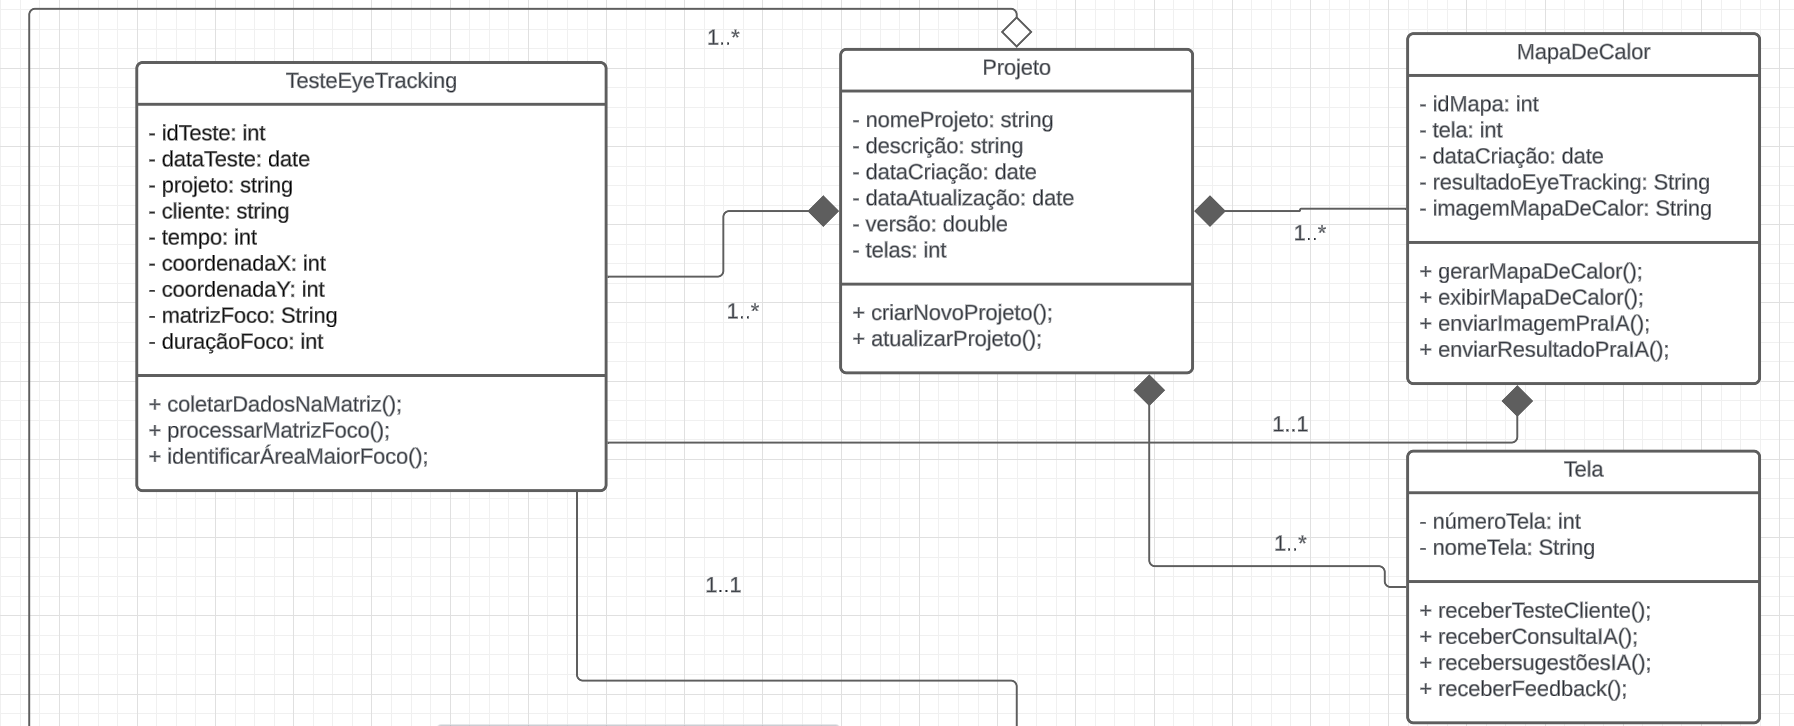
\includegraphics[width = \CaptionWidth]{Illustrations/classes1.png}}
    \usebox0%
    \SourceOrNote{Autoria Própria (2024)}
    \end{photograph}
    
    \vspace{12pt}

    \begin{photograph}[H]
        \centering
        \SetCaptionWidth{\ifbool{@LayoutA}{0.7}{0.72}\linewidth}
        \caption{Diagrama de Classes - Continuação}%
        \label{phot:pg-classes2}
        \savebox0{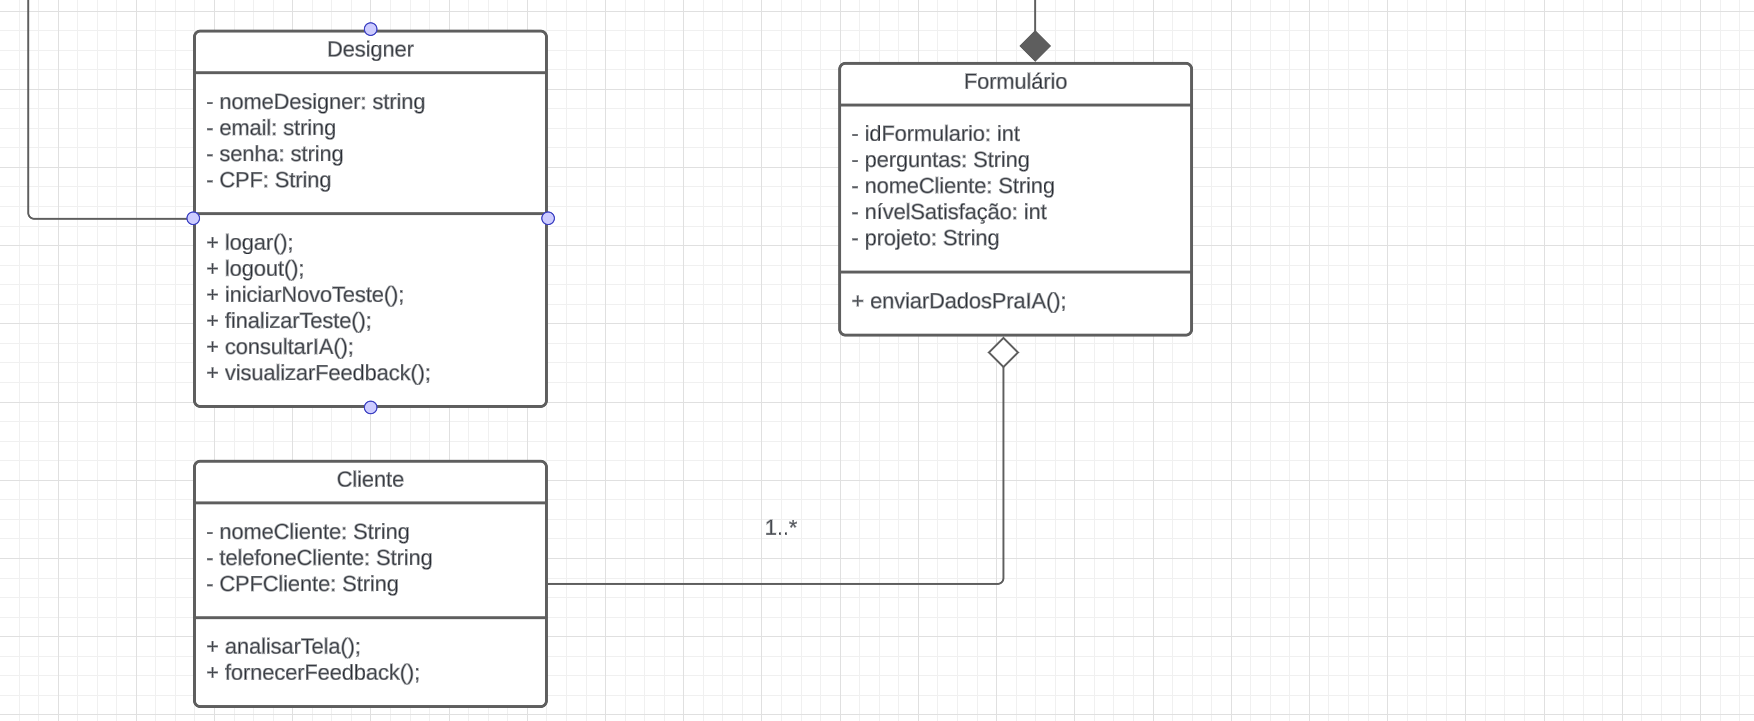
\includegraphics[width = \CaptionWidth]{Illustrations/classes2.png}}
        \usebox0%
        \SourceOrNote{Autoria Própria (2024)}
        \end{photograph}

\subsection*{DIAGRAMA DE OBJETOS}
O diagrama de objetos é uma representação visual que exibe instâncias específicas de classes em um momento particular do sistema, mostrando objetos com seus valores atuais de atributos e as relações entre eles. Diferente do diagrama de classes, que é mais abstrato e define a estrutura geral, o diagrama de objetos detalha uma visão concreta do estado do sistema em determinado instante, facilitando a compreensão das interações entre os objetos e a verificação de como o sistema se comporta na prática.

No diagrama de objetos, as sete instâncias identificadas representam os principais componentes do sistema e como eles interagem em um cenário específico. A instância designer: Designer contém os dados do designer responsável pelo projeto, incluindo nome, e-mail e CPF, enquanto cli: Cliente apresenta as informações do cliente que está avaliando o projeto.

A instância proj: Projeto refere-se ao projeto sendo analisado, com atributos como nome, descrição, data de criação e atualização, e número de telas. Cada tela é representada por uma instância específica, como tela: Tela, que armazena informações detalhadas sobre uma interface específica do projeto.

O teste: TesteEyeTracking registra os dados coletados pelo Eye Tracking, como a matriz de foco e a duração, facilitando a análise do comportamento do usuário. A partir do teste, temos as instâncias form: Formulário e mapa: MapaDeCalor, onde o formulário coleta o feedback do cliente, e o mapa de calor armazena os dados de visualização, oferecendo insights para os UX designers.\newline

\begin{photograph}[H]
    \centering
    \SetCaptionWidth{\ifbool{@LayoutA}{0.7}{0.72}\linewidth}
    \caption{Diagrama de Objetos}%
    \label{phot:pg-objetos}
    \savebox0{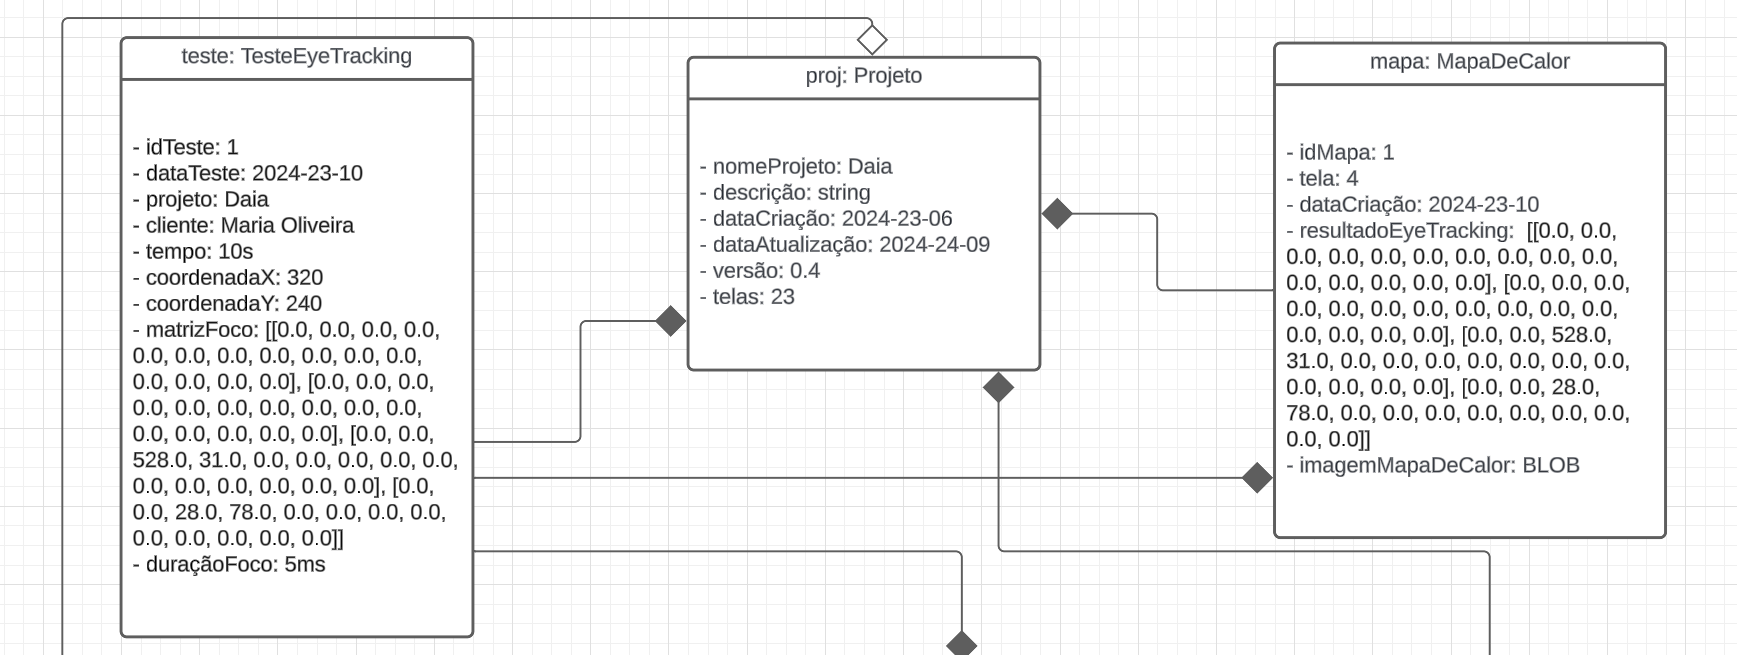
\includegraphics[width = \CaptionWidth]{Illustrations/objetos1.png}}
    \usebox0%
    \SourceOrNote{Autoria Própria (2024)}
    \end{photograph}
    
    \vspace{12pt}

    \begin{photograph}[H]
        \centering
        \SetCaptionWidth{\ifbool{@LayoutA}{0.7}{0.72}\linewidth}
        \caption{Diagrama de Objetos - Continuação}%
        \label{phot:pg-objetos2}
        \savebox0{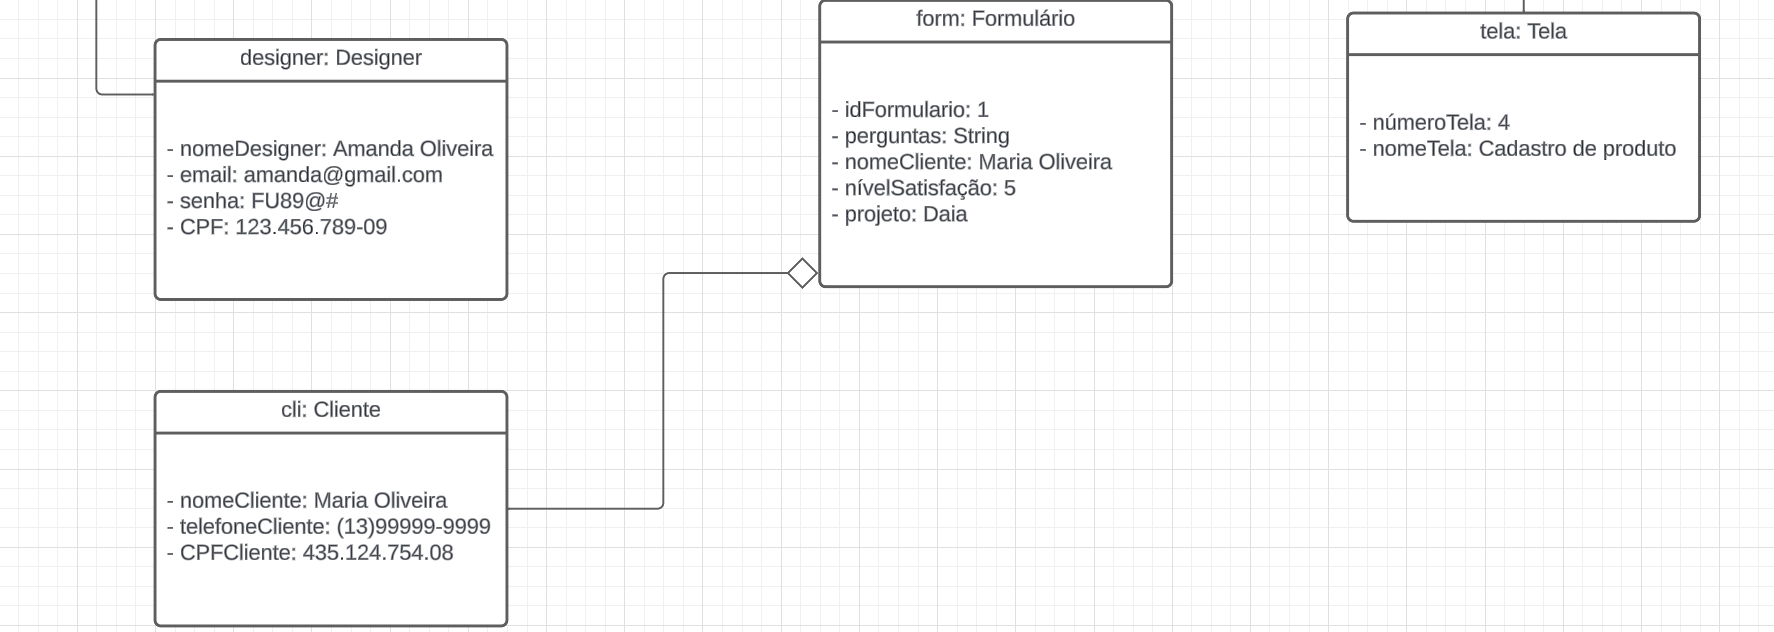
\includegraphics[width = \CaptionWidth]{Illustrations/objetos2.png}}
        \usebox0%
        \SourceOrNote{Autoria Própria (2024)}
        \end{photograph}

\subsection*{BANCO DE DADOS RELACIONAL}
Para construir o modelo físico do banco de dados da aplicação foi utilizada a Linguagem de Consulta Estruturada (SQL) e o MySQL.

A SQL é uma linguagem de programação padronizada usada para gerenciar e manipular dados em bancos de dados relacionais, organizando informações em tabelas de linhas e colunas. Por meio de comandos SQL, é possível inserir, atualizar, excluir e consultar dados no banco, além de realizar otimizações para melhorar seu desempenho.

O MySQL, por sua vez, é um sistema de gerenciamento de banco de dados relacional de código aberto, mantido pela Oracle, que utiliza a SQL como base para suas operações. É amplamente usado em aplicações web e pode ser instalado em sistemas operacionais diversos, assim como em servidores de nuvem. \textcite{Amazon}\newline

\subsection*{PROTOTIPAÇÃO DO SOFTWARE UEYE}
A (\Cref{phot:pg-tela1}) representa a tela inicial do designer. Logo após fazer o login, o mesmo tem acesso a todos os seus projetos podendo decidir qual manipular.

\begin{photograph}[H]
    \centering
    \SetCaptionWidth{\ifbool{@LayoutA}{0.7}{0.72}\linewidth}
    \caption{Tela 1}%
    \label{phot:pg-tela1}
    \savebox0{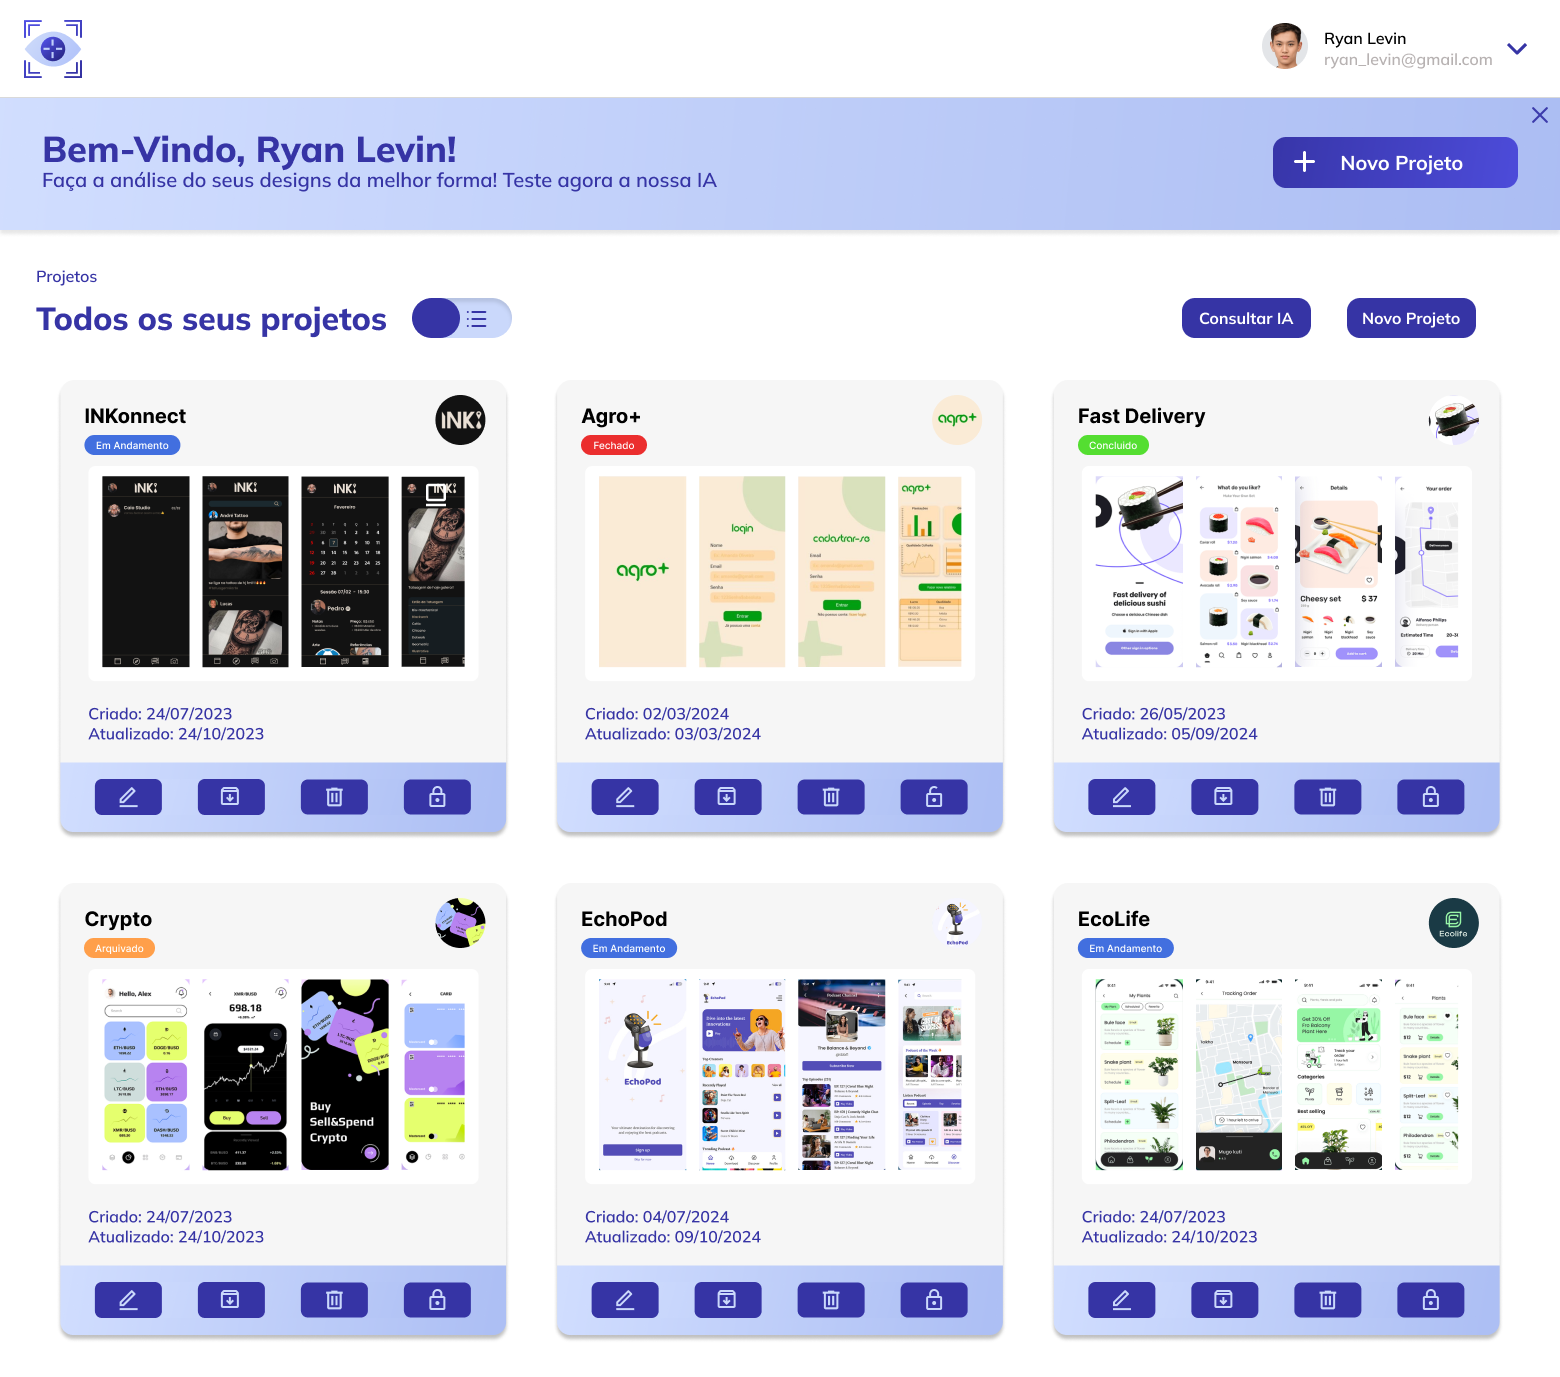
\includegraphics[width = \CaptionWidth]{Illustrations/tela1.png}}
    \usebox0%
    \SourceOrNote{Autoria Própria (2024)}
    \end{photograph}

A (\Cref{phot:pg-tela2}) representa a tela que o designer tem acesso ao entrar em um projeto. Nela é possível visualizar as telas pertencentes ao projeto, assim como dois gráficos. O da esquerda representa o número de notas baixas atribuídas a esse projeto de acordo com três quesitos. Por exemplo, o projeto em específico obteve trinta e cinco notas baixas no quesito “Atratividade visual”. Enquanto o gráfico da direita ilustra a taxa de satisfação por avaliação através da IA por períodos de tempo, nesse caso, dias. Além disso é possível clicar nos botões de “Consultar IA” e no de “Eye-tracking”, onde no último é possível escolher entre fazer um novo teste ou visualizar as avalições anteriores de clientes. 

\begin{photograph}[H]
    \centering
    \SetCaptionWidth{\ifbool{@LayoutA}{0.7}{0.72}\linewidth}
    \caption{Tela 2}%
    \label{phot:pg-tela2}
    \savebox0{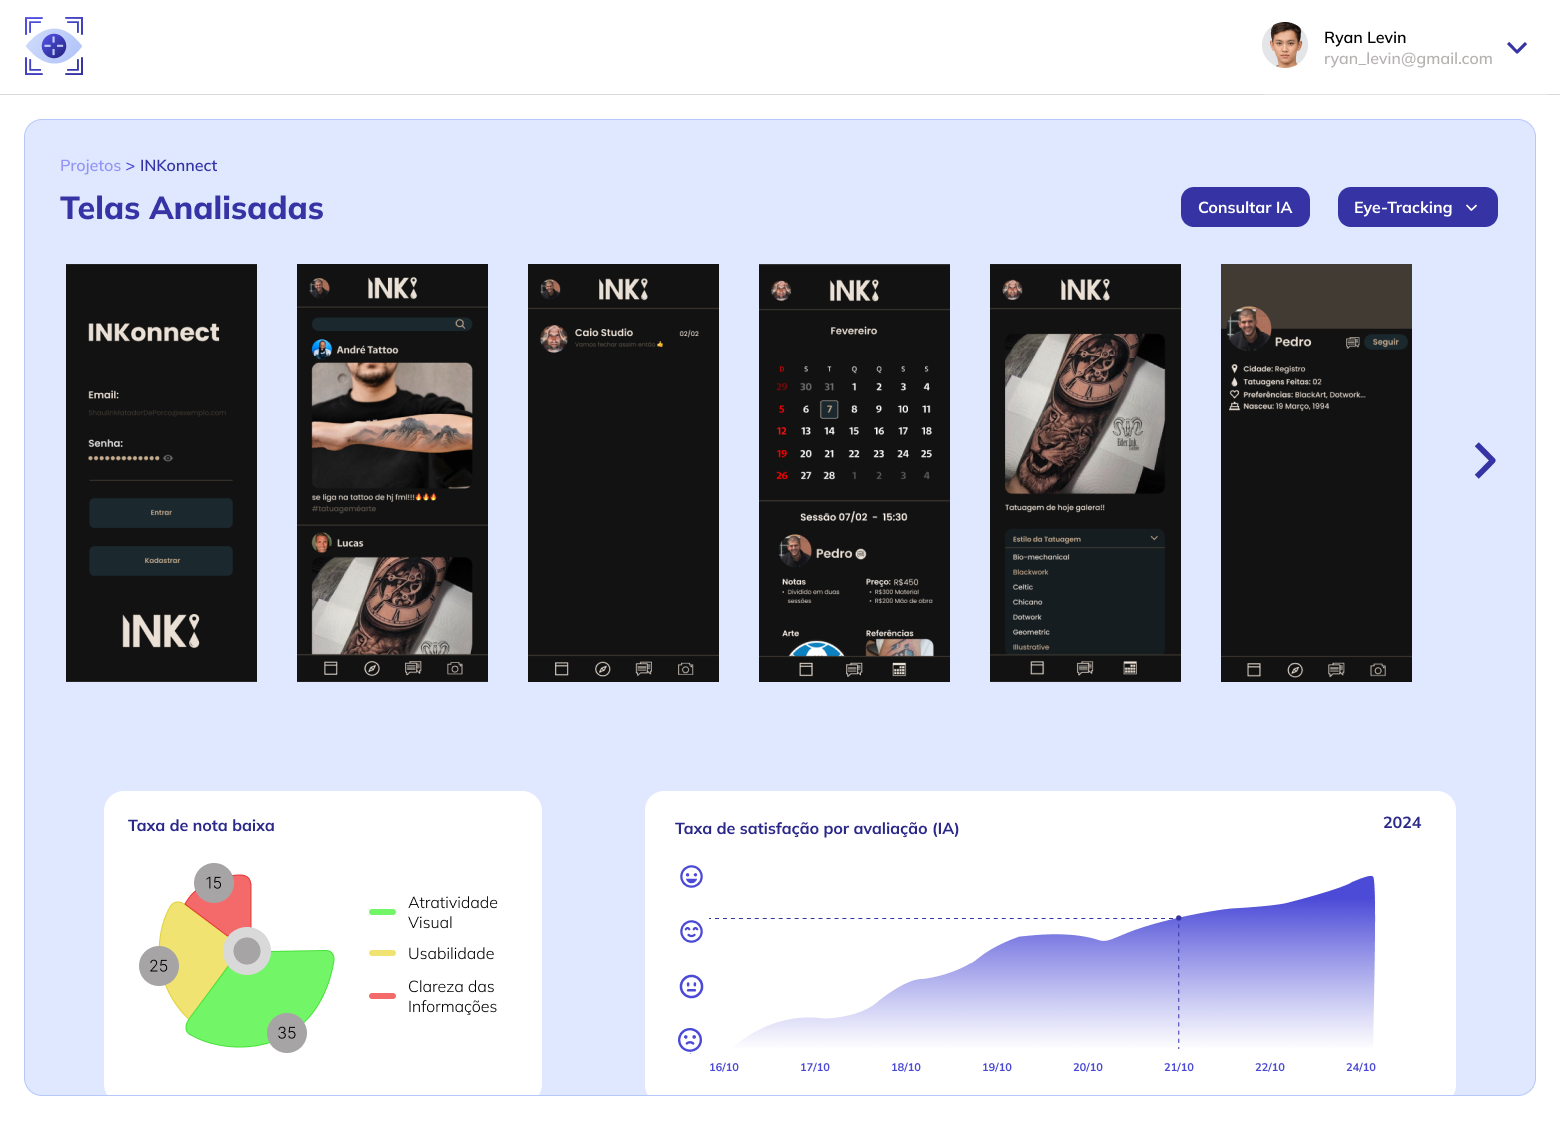
\includegraphics[width = \CaptionWidth]{Illustrations/tela2.png}}
    \usebox0%
    \SourceOrNote{Autoria Própria (2024)}
    \end{photograph}

Na (\Cref{phot:pg-tela3}), observa-se que, ao clicar em uma das telas do projeto, o usuário pode acessar o histórico de avaliações realizadas pela IA.

\begin{photograph}[H]
    \centering
    \SetCaptionWidth{\ifbool{@LayoutA}{0.7}{0.72}\linewidth}
    \caption{Tela 3}%
    \label{phot:pg-tela3}
    \savebox0{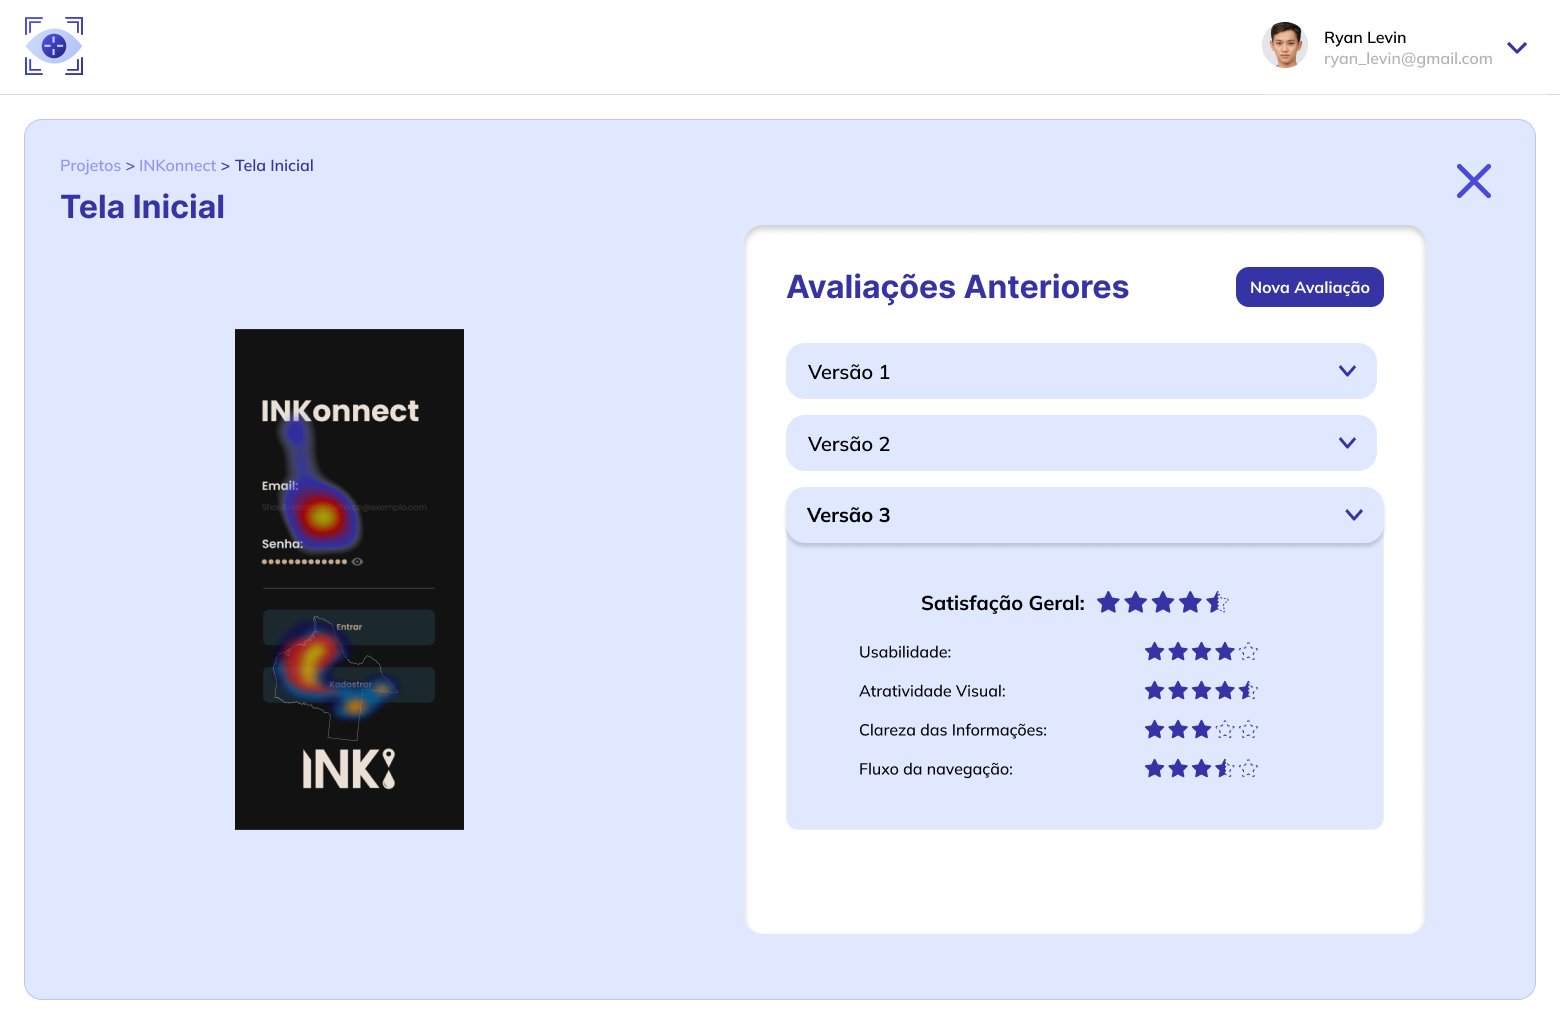
\includegraphics[width = \CaptionWidth]{Illustrations/tela3.png}}
    \usebox0%
    \SourceOrNote{Autoria Própria (2024)}
    \end{photograph}

Ao clicar no botão “Consultar IA” da \Cref{phot:pg-tela2}, o designer tem acesso a janela (\Cref{phot:pg-tela4}) em que é possível carregar uma tela do projeto para que a IA faça a avaliação da mesma. 

\begin{photograph}[H]
    \centering
    \SetCaptionWidth{\ifbool{@LayoutA}{0.7}{0.72}\linewidth}
    \caption{Tela 4}%
    \label{phot:pg-tela4}
    \savebox0{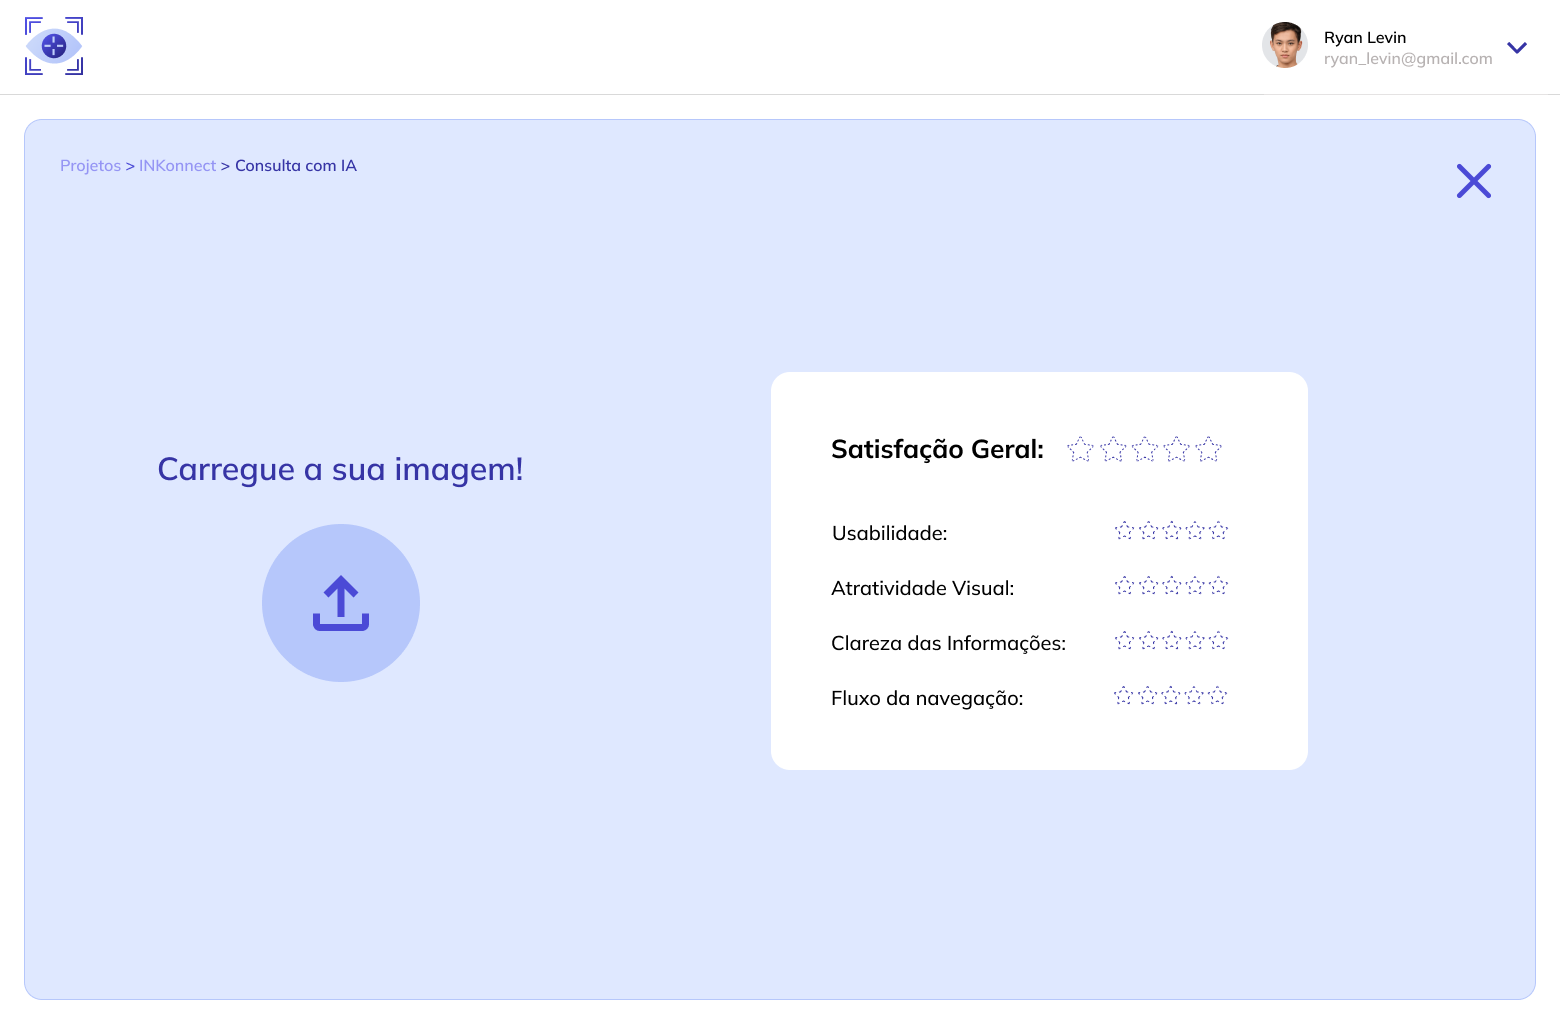
\includegraphics[width = \CaptionWidth]{Illustrations/tela4.png}}
    \usebox0%
    \SourceOrNote{Autoria Própria (2024)}
    \end{photograph}

A (\Cref{phot:pg-tela5}) ilustra a tela do projeto após receber a avaliação da IA. 

\begin{photograph}[H]
    \centering
    \SetCaptionWidth{\ifbool{@LayoutA}{0.7}{0.72}\linewidth}
    \caption{Tela 5}%
    \label{phot:pg-tela5}
    \savebox0{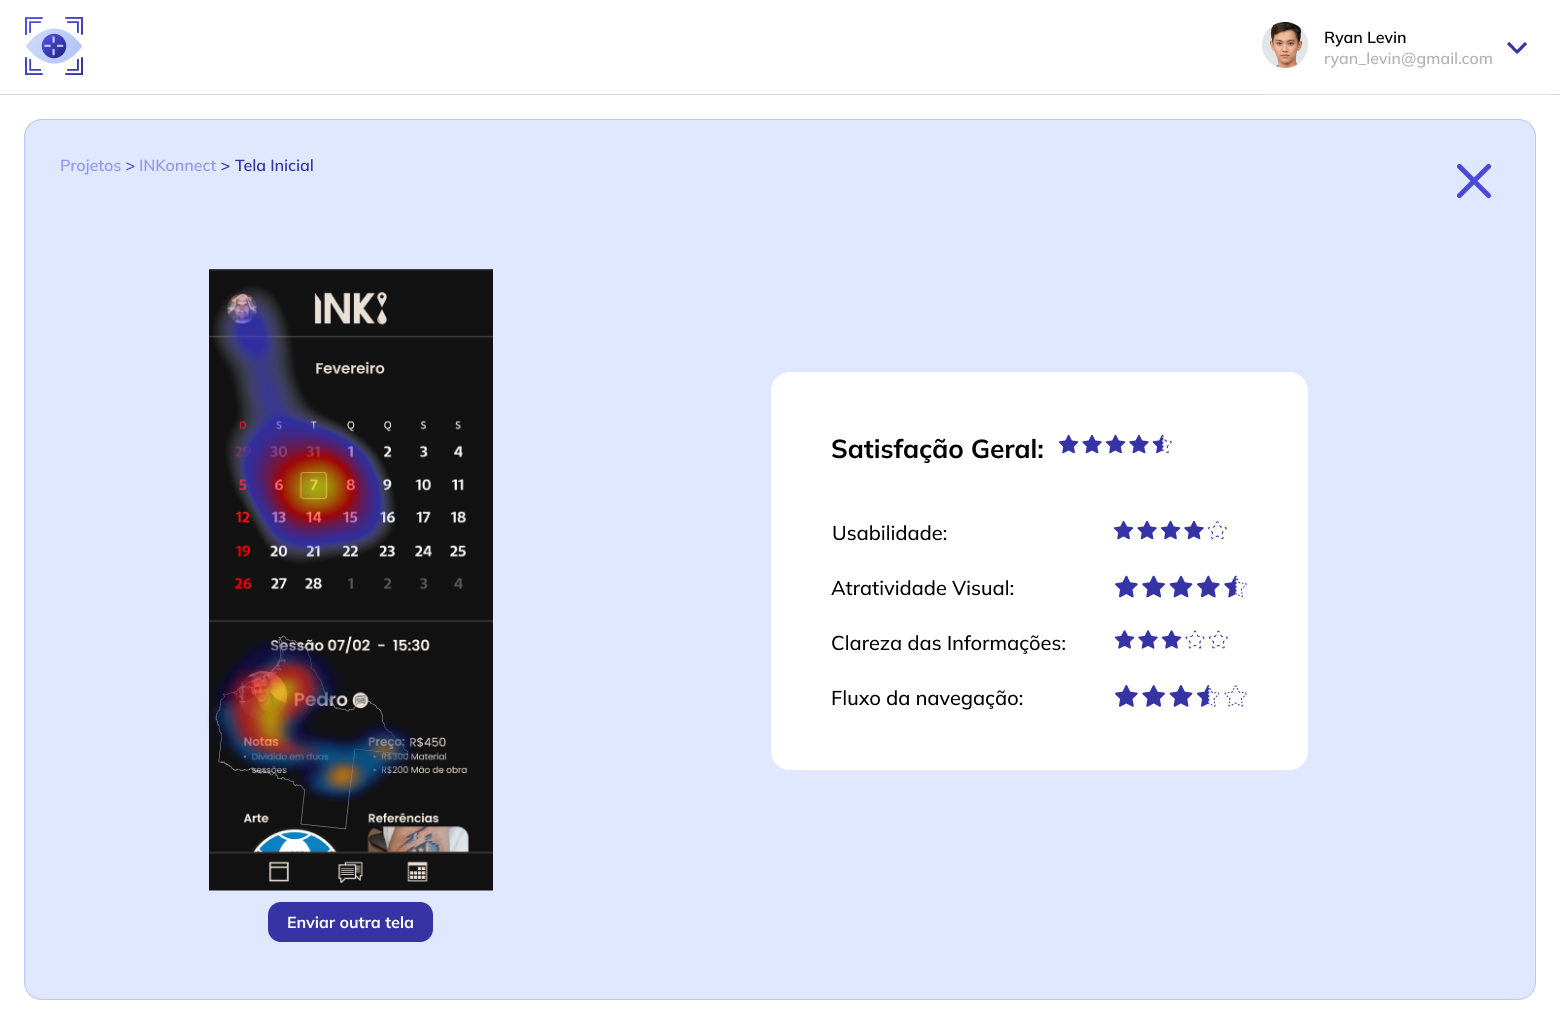
\includegraphics[width = \CaptionWidth]{Illustrations/tela5.png}}
    \usebox0%
    \SourceOrNote{Autoria Própria (2024)}
    \end{photograph}

Ao selecionar a opção de fazer um novo teste na (\Cref{phot:pg-tela2}), o cliente deve colocar suas informações pessoais para iniciar o teste (\Cref{phot:pg-tela6}). 

\begin{photograph}[H]
    \centering
    \SetCaptionWidth{\ifbool{@LayoutA}{0.7}{0.72}\linewidth}
    \caption{Tela 6}%
    \label{phot:pg-tela6}
    \savebox0{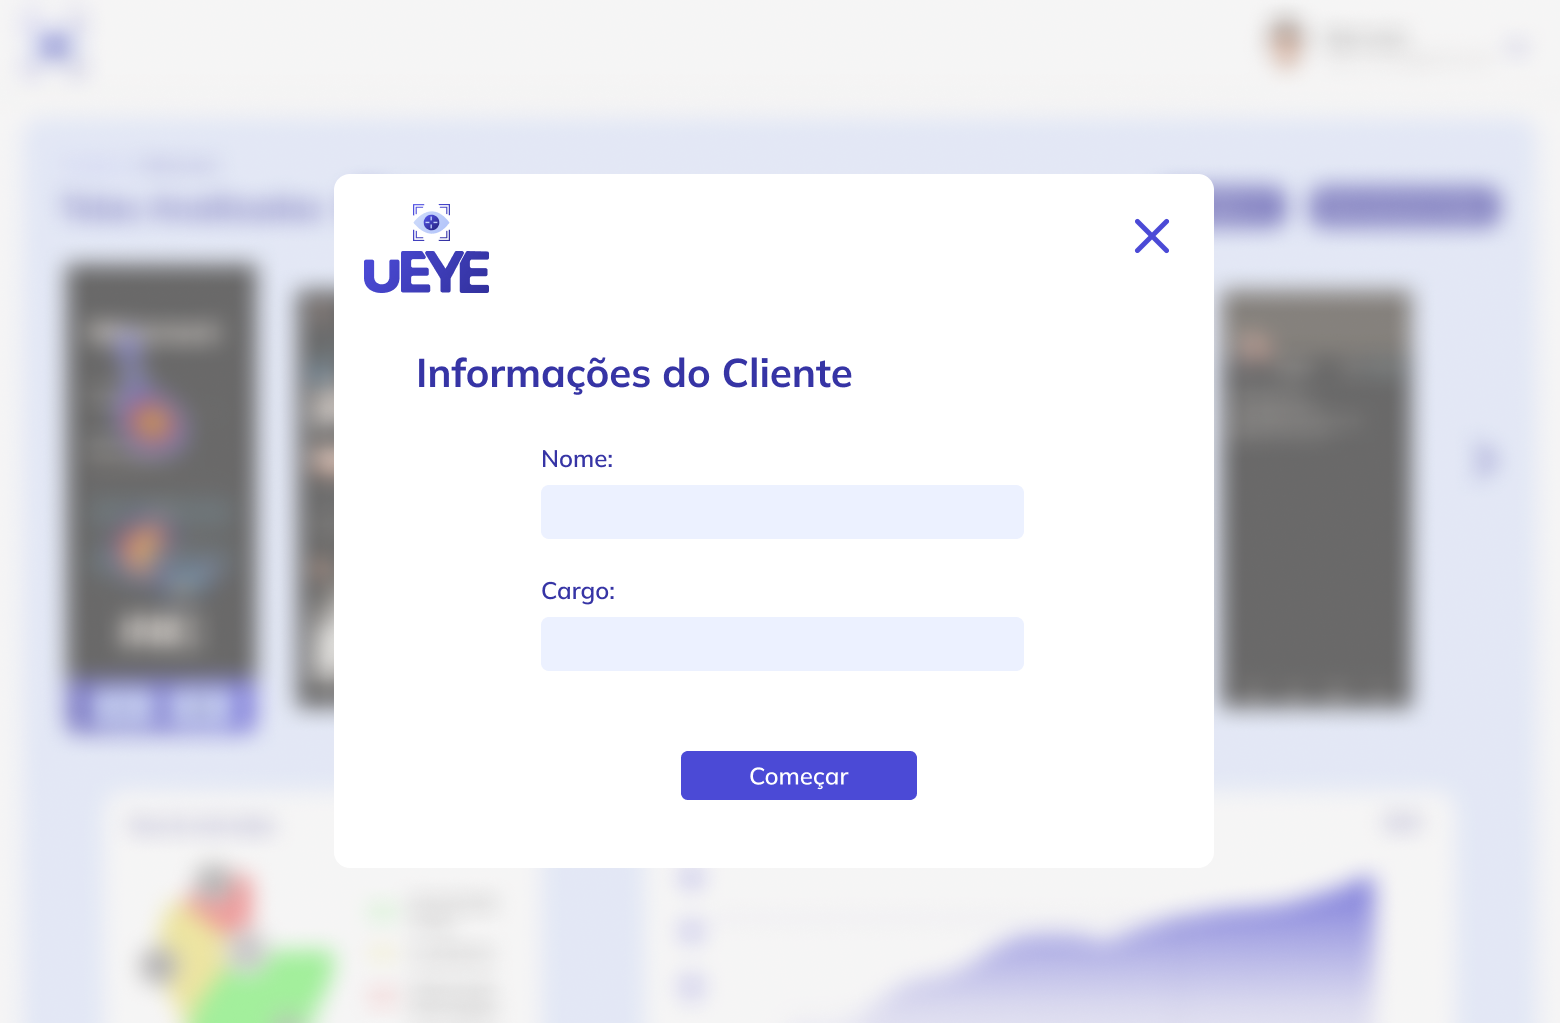
\includegraphics[width = \CaptionWidth]{Illustrations/tela6.png}}
    \usebox0%
    \SourceOrNote{Autoria Própria (2024)}
    \end{photograph}

A (\Cref{phot:pg-tela7}) ilustra o design sendo exibido ao cliente enquanto ele faz o Eye Tracking. 

\begin{photograph}[H]
    \centering
    \SetCaptionWidth{\ifbool{@LayoutA}{0.7}{0.72}\linewidth}
    \caption{Tela 7}%
    \label{phot:pg-tela7}
    \savebox0{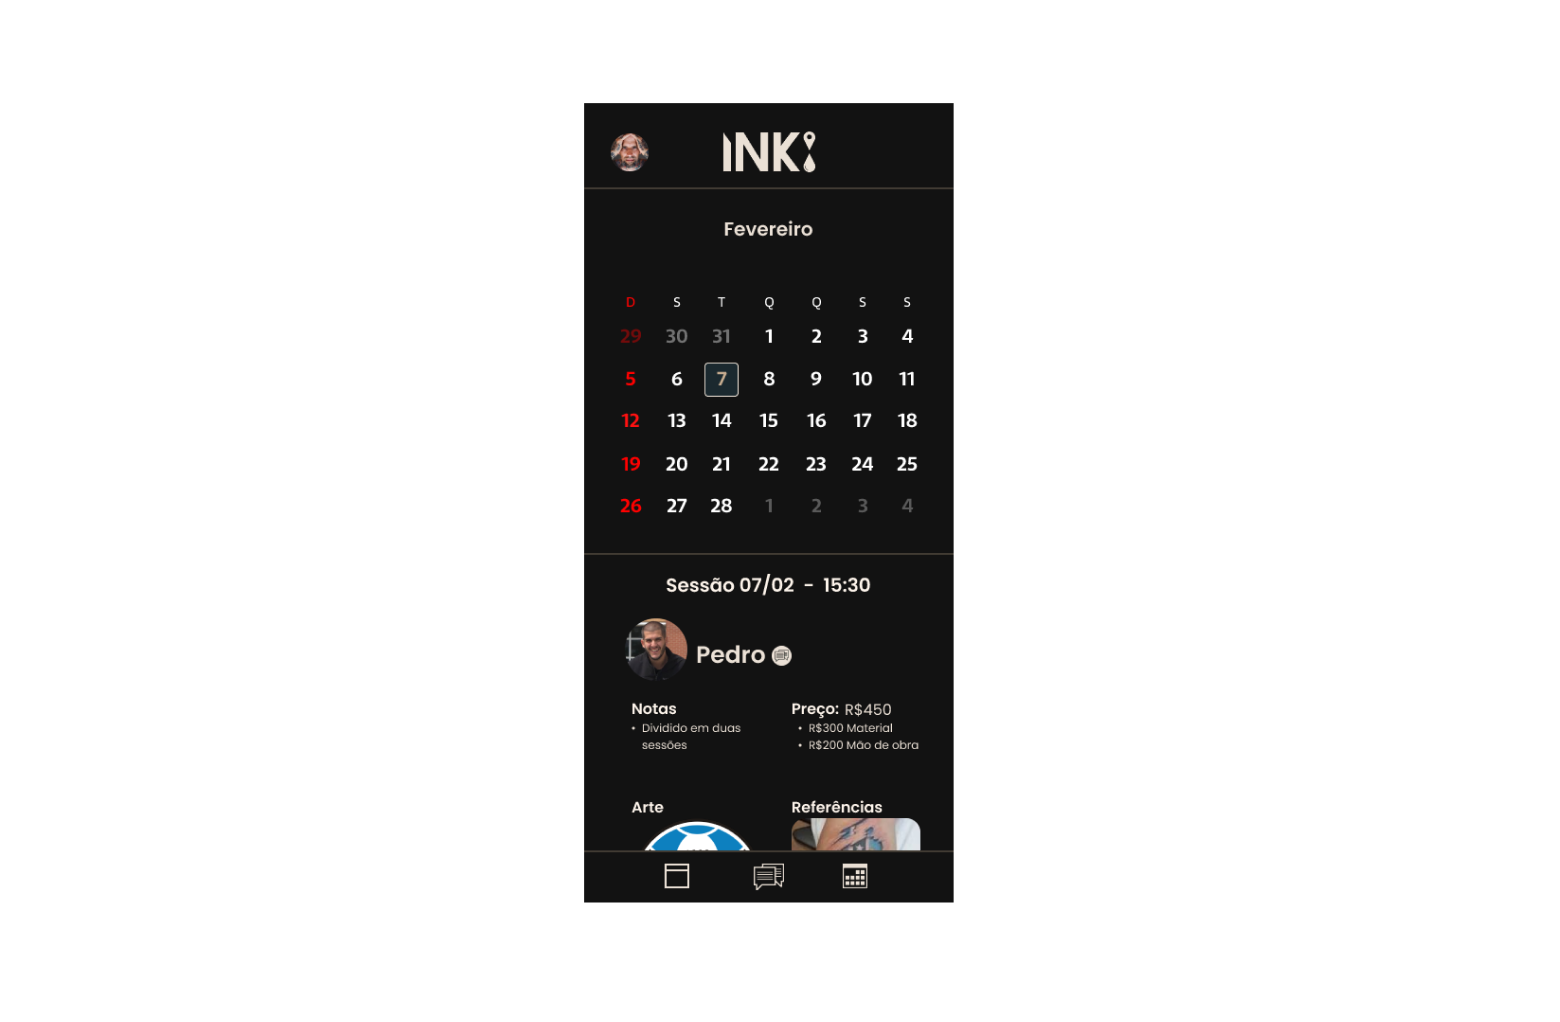
\includegraphics[width = \CaptionWidth]{Illustrations/tela7.png}}
    \usebox0%
    \SourceOrNote{Autoria Própria (2024)}
    \end{photograph}

Após o teste, a tela (\Cref{phot:pg-tela8}) a seguir será exibida ao cliente para que ele forneça o devido feedback, dados os quais serão utilizados para retroalimentar a IA. 

\begin{photograph}[H]
    \centering
    \SetCaptionWidth{\ifbool{@LayoutA}{0.7}{0.72}\linewidth}
    \caption{Tela 8}%
    \label{phot:pg-tela8}
    \savebox0{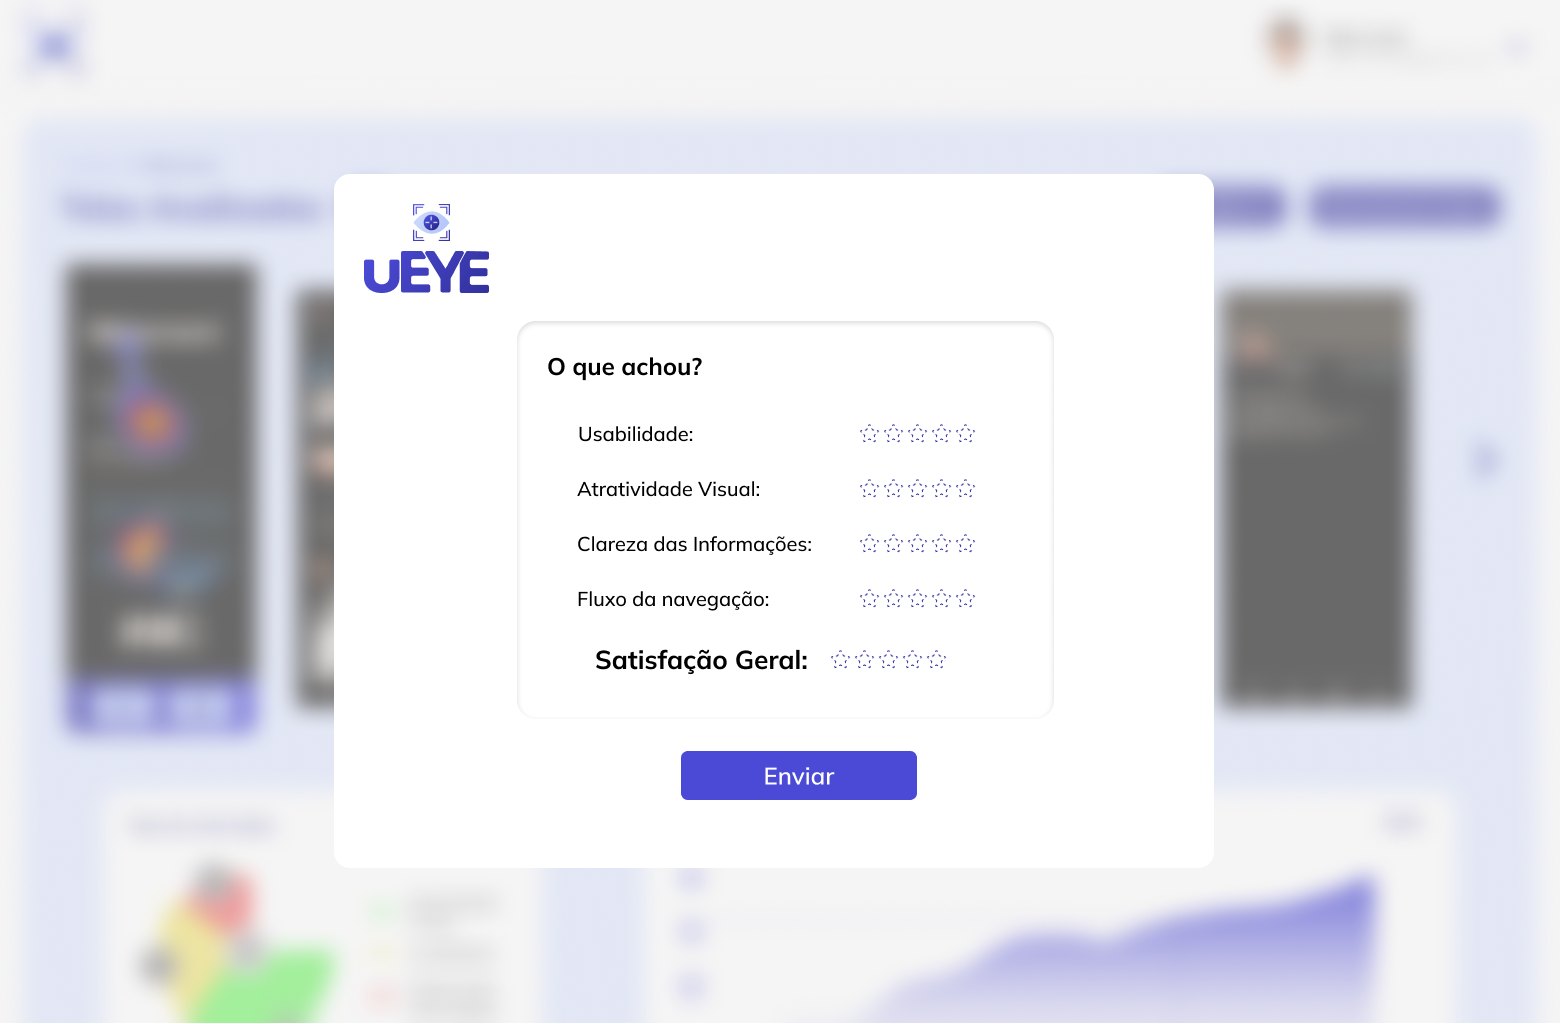
\includegraphics[width = \CaptionWidth]{Illustrations/tela8.png}}
    \usebox0%
    \SourceOrNote{Autoria Própria (2024)}
    \end{photograph}

Ao selecionar o botão “Ver avaliações” na (\Cref{phot:pg-tela2}), o designer tem acesso ao histórico de avaliações dos clientes, como na imagem a seguir. 

\begin{photograph}[H]
    \centering
    \SetCaptionWidth{\ifbool{@LayoutA}{0.7}{0.72}\linewidth}
    \caption{Tela 9}%
    \label{phot:pg-tela9}
    \savebox0{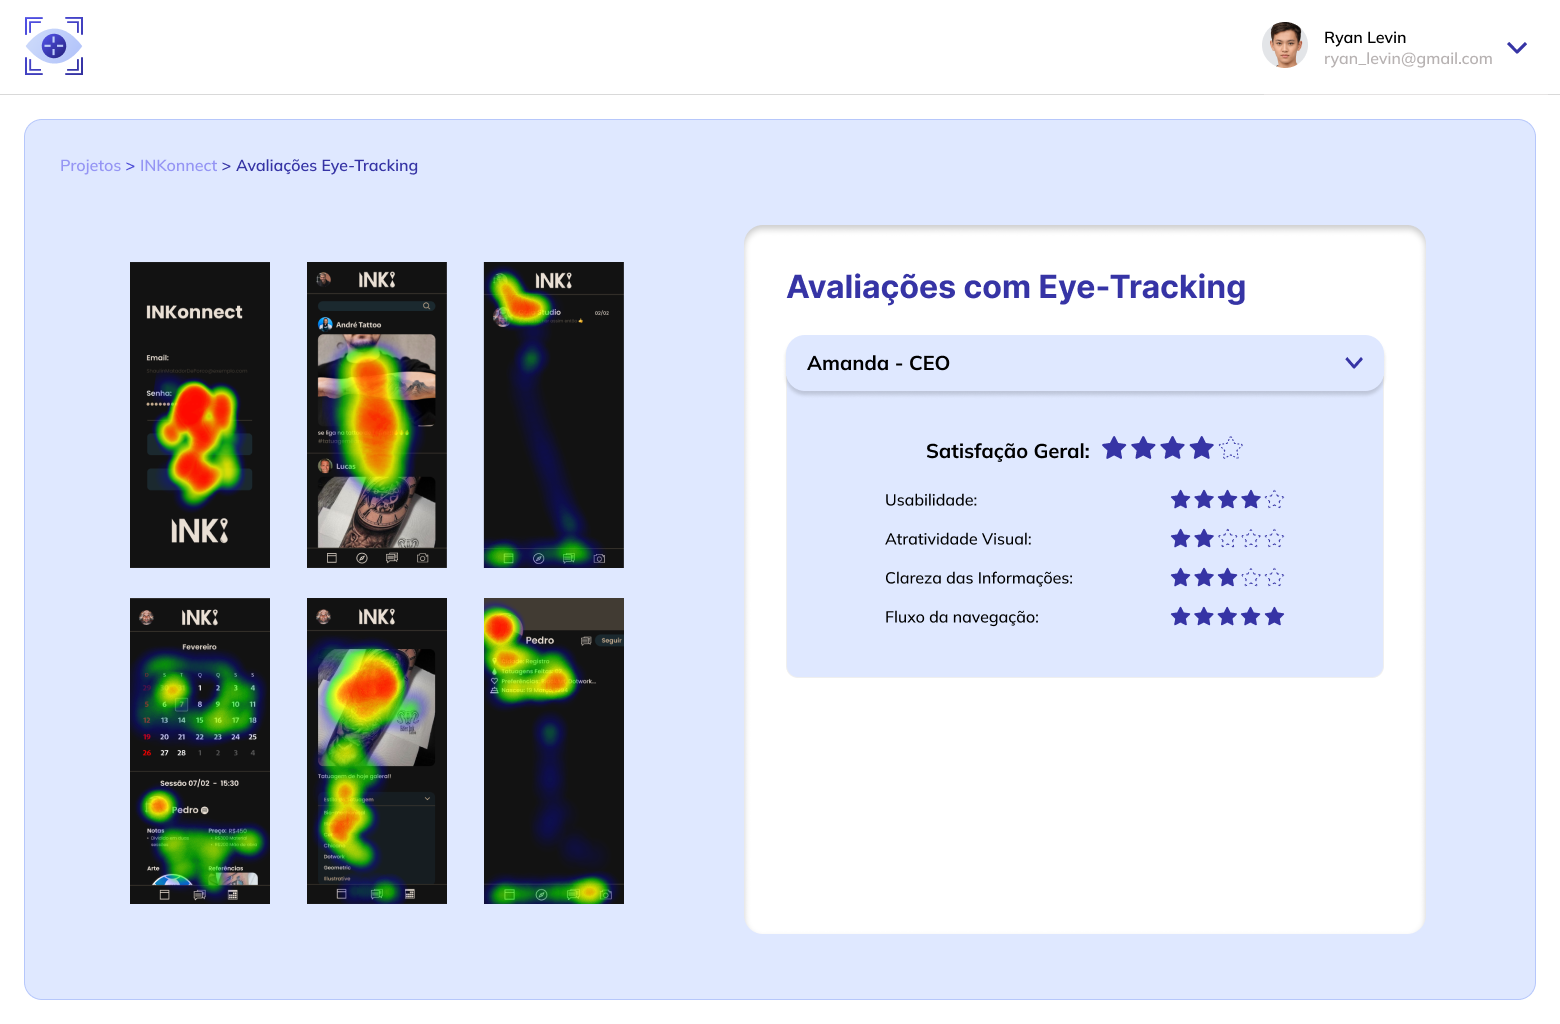
\includegraphics[width = \CaptionWidth]{Illustrations/tela9.png}}
    \usebox0%
    \SourceOrNote{Autoria Própria (2024)}
    \end{photograph}

\section*{CONCLUSÃO}\label{sect:conclusao}

Para auxiliar no cumprimento dos Objetivos de Desenvolvimento Sustentável (ODS), estabelecidos pela Organização das Nações Unidas (ONU), o projeto atual busca contribuir para o nono objetivo, que promove a Inovação e a Infraestrutura, ao desenvolver uma nova abordagem para a análise do design de interfaces de usuário. \textcite{ODS2024}

O sistema será desenvolvido para apoiar designers de UX, integrando Eye Tracking, Heatmaps e Inteligência Artificial, com o objetivo de otimizar o processo de validação de interfaces. A ferramenta permitirá que o designer envie telas para análise preditiva da IA, que retornará um heatmap e uma escala de satisfação baseados em critérios como usabilidade e fluxo de navegação. O sistema registra dados de rastreamento ocular durante os testes, gerando um modelo preditivo para análises futuras, eliminando a necessidade de repetição de testes com usuários reais. Assim, a ferramenta visa agilizar o processo de design, mantendo a qualidade da interface por meio de análises automatizadas.

Todo o processo será realizado por meio do software uEye, que integrará tanto o Eye Tracking quanto a consulta à Inteligência Artificial.

Até o momento, alcançamos a integração bem-sucedida de bibliotecas como OpenCV e MediaPipe para realizar a detecção facial e ocular, bem como a geração de mapas de calor utilizando PyGame e Matplotlib. O sistema está em funcionamento, coletando dados de interação dos usuários. O banco de dados relacional desenvolvido com MySQL está estruturado para armazenar informações sobre os testes de rastreamento ocular, possibilitando o treinamento futuro da IA por meio de consultas em tempo real.

Ao analisar os artefatos do projeto, percebe-se que o estudo atual ainda demanda testes práticos em contextos reais com profissionais especializados, a fim de obter relatórios e avaliações que possibilitem a melhoria contínua do sistema. Além disso, há a necessidade de realizar estudos mais intensivos sobre Testes de Usabilidade e Eye Tracking para aprimorar a precisão dos dados fornecidos, especialmente no que se refere ao rastreamento ocular. Esses testes também fornecerão um retorno valioso sobre a eficácia e usabilidade da análise preditiva de modelos de UX de alta fidelidade orientados pelo rastreamento ocular.

No que se refere à identificação dos dados de forma intuitiva em mapas de calor, propõe-se o uso do processo de homogenização. Nesse processo, as áreas de foco visual do usuário receberão um valor estimado, criando uma representação contínua dos dados, suavizando as variações e permitindo uma visualização aprimorada das regiões de maior concentração visual.

Espera-se que a expansão do sistema para incluir a consulta preditiva da IA, sem a necessidade de novos testes com usuários reais, otimize o fluxo de trabalho dos designers, garantindo que a interface seja constantemente aprimorada com base em análises automatizadas. Espera-se, ainda, que o sistema auxilie os designers de UX tanto na análise preditiva quanto na precisão dos dados obtidos para o treinamento da IA. Cabe destacar que as novas tecnologias a serem incluídas futuramente têm o potencial de ser reconhecidas como fatores cruciais para a eficácia do projeto.

\printbibliography

%% Elementos pós-textuais (opcionais): Apêndice e Anexo
%Caso for utilizar, basta retirar o símbolo de % na frente do comando
%%%%% Elementos pós-textuais
%%
%% Glossário, apêndices, anexos e índice remissivo (opcionais).

%% Apêndices
\begin{Appendix}

\section{Título de Apêndice}%
\label{sect:apx-a1}

Exemplo de apêndice (\Cref{sect:apx-a1}) em uma seção de \nameref{sect:appendix}.

\subsection{Título de Seção Secundária de Apêndice}%
\label{ssect:apx-a2}

Exemplo de seção secundária de apêndice (\Cref{ssect:apx-a2}).

\subsubsection{Título de Seção Terciária de Apêndice}%
\label{sssect:apx-a3}

Exemplo de seção terciária de apêndice (\Cref{sssect:apx-a3}).

\paragraph{Título de seção quaternária de Apêndice}%
\label{prgh:apx-a4}

Exemplo de seção quaternária de apêndice (\Cref{prgh:apx-a4}).

\subparagraph{Título de seção quinária de Apêndice}%
\label{sprgh:apx-a5}

Exemplo de seção quinária de apêndice (\Cref{sprgh:apx-a5}).

\end{Appendix}

%% Anexos
\begin{Annex}

\section{Título de Anexo}%
\label{sect:anx-a1}

Exemplo de anexo (\Cref{sect:anx-a1}) em uma seção de \nameref{sect:annex}.

\subsection{Título de Seção Secundária de Anexo}%
\label{ssect:anx-a2}

Exemplo de seção secundária de anexo (\Cref{ssect:anx-a2}).

\subsubsection{Título de Seção Terciária de Anexo}%
\label{sssect:anx-a3}

Exemplo de seção terciária de anexo (\Cref{sssect:anx-a3}).

\paragraph{Título de seção quaternária de Anexo}%
\label{prgh:anx-a4}

Exemplo de seção quaternária de anexo (\Cref{prgh:anx-a4}).

\subparagraph{Título de seção quinária de Anexo}%
\label{sprgh:anx-a5}

Exemplo de seção quinária de anexo (\Cref{sprgh:anx-a5}).

\end{Annex}

%% Índice remissivo
\printindex%


%% Fim do documento
\end{document}